\subsection{Architettura backend}
\subsubsection{Elenco dei componenti}
Per lo sviluppo del backend verrà utilizzato il framework NestJS, il backend verrà infatti suddiviso in moduli, controller e provider.

\paragraph{Moduli}
I moduli vengono definiti utilizzando il decoratore \texttt{@Module} fornito da NestJS.
Un modulo raggruppa provider, controller ed eventuali dipendenze condivise tra più parti dell'applicazione.
\begin{itemize}
    \item \textbf{AppModule}: modulo principale dell'applicazione, importa altri moduli, definisce i controller da esporre e fornisce i servizi necessari, raggruppa e organizza il backend in componenti riutilizzabili;
    \item \textbf{DataSourceModule}: responsabile della logica per il recupero dei dati necessari per fornire all'utente la descrizione dei dataset che saranno disponibili nell'applicazione;
    \begin{figure}[h!] \centering       
        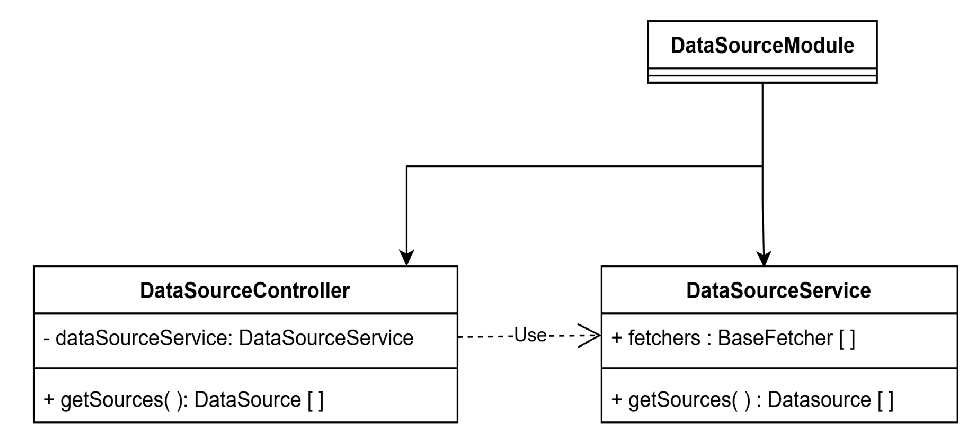
\includegraphics[scale = 0.5]{template/images/uml_back/DataSourceModule.png}
        \caption{DataSourceModule}
    \end{figure}
    \item \textbf{DataVisualizationModule}: incapsula la logica relativa alla trasformazione dei dati ricevuti dalle fonti e li prepara per la visualizzazione nel grafico 3D. Include il controller e il service relativi alla gestione dei dati per la visualizzazione;
    \begin{figure}[h!] \centering       
        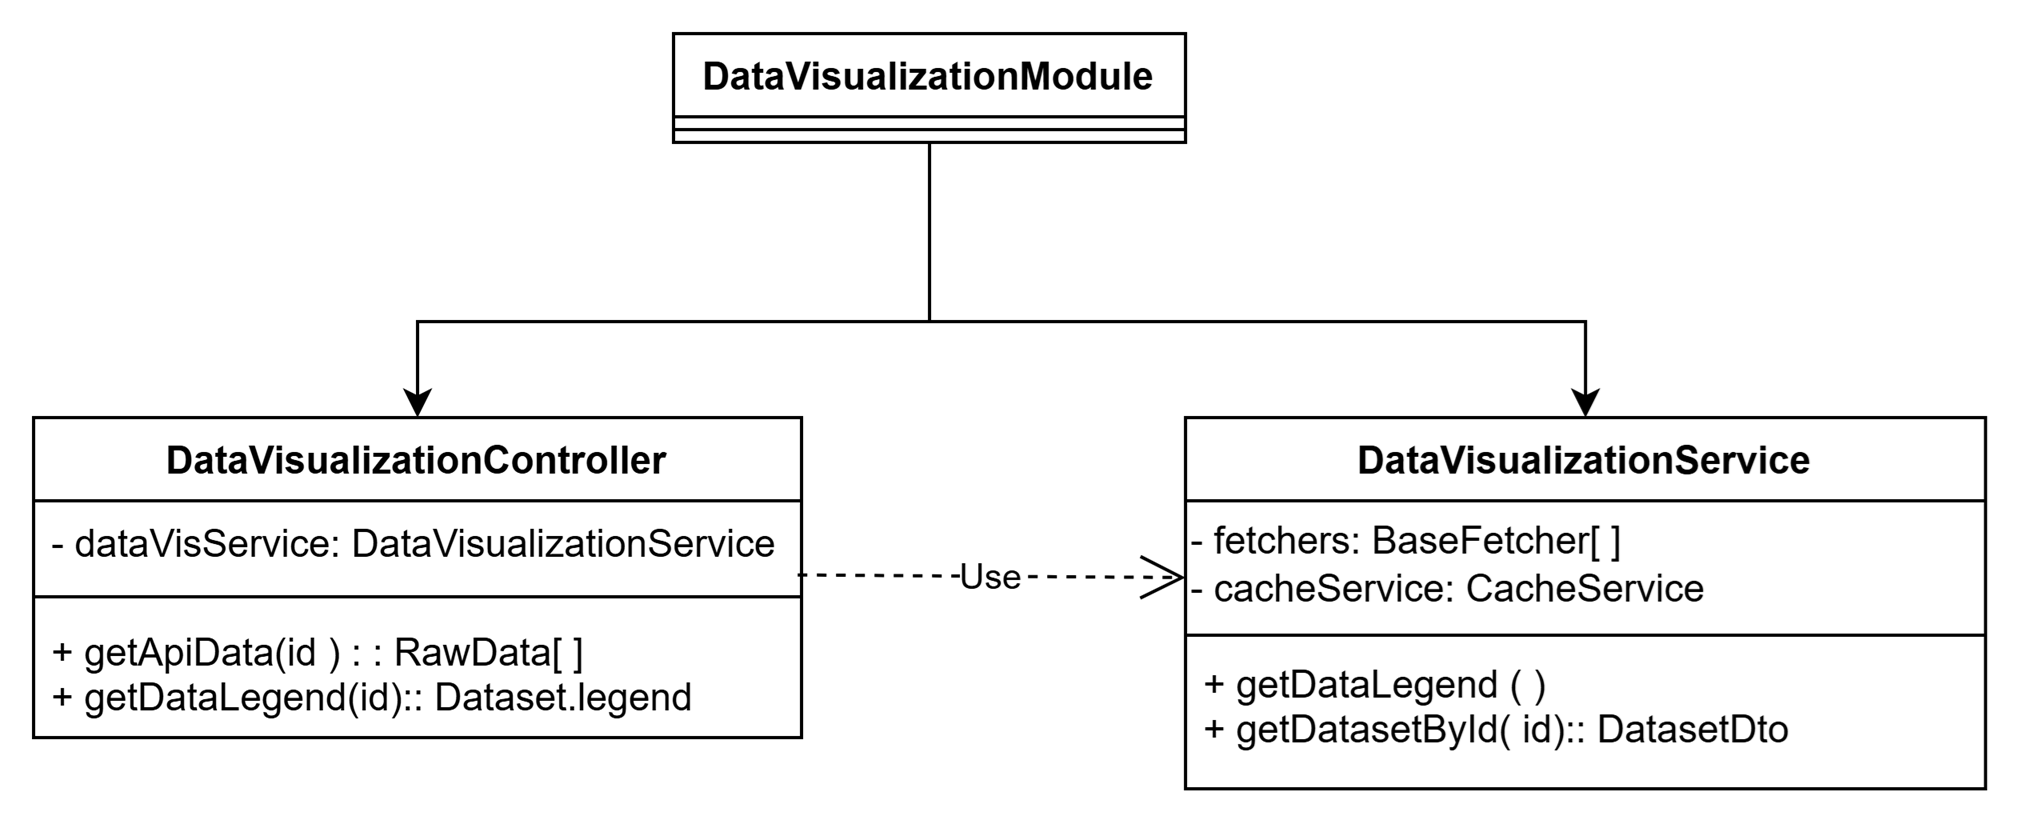
\includegraphics[scale = 0.3]{template/images/uml_back/DataVisualizationModule.png}
        \caption{DataVisualizationModule}
    \end{figure}
    \newpage
    \item \textbf{CacheModule}: responsabile della gestione della cache lato server, utilizza Memcached per memorizzare temporaneamente i dati richiesti da fetcher al fine di ridurre il carico sulle API esterne e migliorare le performance.
    \begin{figure}[h!] \centering       
        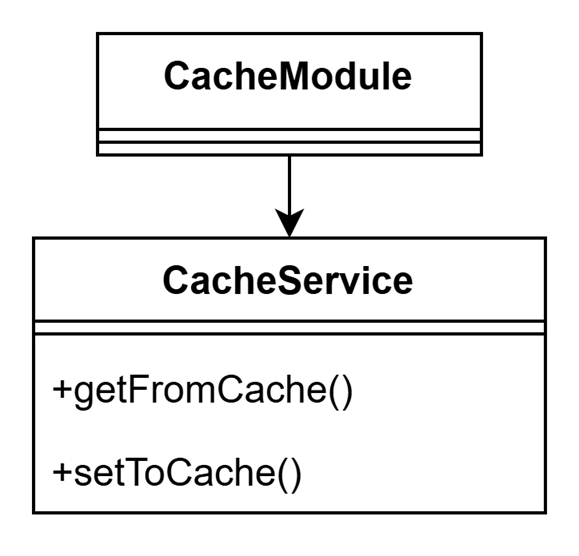
\includegraphics[scale = 0.3]{template/images/uml_back/CacheModule.png}
        \caption{CacheModule}
    \end{figure}
\end{itemize}

\paragraph{Controller}
I controller vengono definiti utilizzando il decoratore \texttt{@Controller} fornito da NestJs.
Un controller gestisce le richieste HTTP in arrivo e invia le risposte al client da parte del backend.
\begin{itemize}
    \item \textbf{AppController}: gestisce le richieste HTTP in arrivo, esponendo endpoint, chiama metodi del Service per ottenere i dati o eseguire logiche, automaticamente, grazie al dependency injection;
    \item \textbf{DataSourceController}: espone un endpoint HTTP GET e utilizza il servizio \textit{DataSourceService} per recuperare la lista delle fonti dati disponibili;
    \begin{itemize}
        \item \textbf{Dipendenze}:
        \begin{itemize}
            \item \textit{DataSourceService}: iniettato nel controller tramite il costruttore, viene utilizzato per ottenere i dati esposti dall'endpoint \texttt{GET /data-source};
            \item \textit{DataSourceDto}: tipo restituito dal metodo \textit{getSources()}, non iniettato, ma utilizzato come dipendenza statica per la tipizzazione della risposta.
        \end{itemize}
    \end{itemize}
    \item \textbf{DataVisualizationController}: espone endpoint per ottenere dataset i dati formattati a partire da una determinata fonte dati. Chiama il \textit{DataVisualizationService}, che si occupa di recuperare il dataset;
    \begin{itemize}
        \item \textbf{Dipendenze}:
        \begin{itemize}
            \item \textit{DataVisualizationService}: è iniettato nel controller tramite il costruttore; il servizio contiene la logica per recuperare i dataset tramite il metodo \texttt{getDatasetById()};
            \item \textit{DatasetDto}: è il tipo che viene restituito nel metodo \texttt{getSources()}, non è iniettato, ma è una dipendenza statica utilizzata per la tipizzazione della risposta.
        \end{itemize}
    \end{itemize}
\end{itemize}

\paragraph{Provider}
Un provider viene definito come una classe con il decoratore \texttt{@Injectable}, che permette a NestJS di gestirlo come un'istanza singleton e di iniettarlo in altri componenti.
Sono classi iniettate tramite il sistema di dependency injection di NestJS. Servono per incapsulare la logica di business.
\begin{itemize}
    \item \textbf{AppService}: contiene la logica di business dell'app, fornisce dati o elabora logiche chiamate dal controller, e a sua volta può accedere ad altri servizi;
    \item \textbf{DataSourceService}: contiene la logica per costruire la lista di \textit{DataSource}, contenenti le informazioni da mostrare all'utente, riceve un array di oggetti \textit{BaseFetcher} tramite injection del token FETCHERS e crea una lista di oggetti \textit{DataSource} mappandoli;
    \begin{itemize}
        \item \textbf{Dipendenze}:
        \begin{itemize}
            \item \textit{BaseFetcher}: dipendenza iniettata tramite il token \texttt{"FETCHERS"}, necessaria per utilizzare il metodo \texttt{fetchData}, in modo da reperire i dati tramite chiamata all'API;
            \item \textit{CacheService}: crea un'istanza per usare il metodo \texttt{getFromCache()} per il reperimento dei dati dalla cache;
        \end{itemize}
    \end{itemize}
    
    \item \textbf{DataVisualizationService}: riceve richieste per il dataset che si desidera visualizzare, gestendo la logica per chiamare la classe \textit{BaseFetcher} per il recupero e la trasformazione dei dati. Se i dati sono già presenti nella cache, li recupera direttamente da essa.
    \begin{itemize}
        \item \textbf{Dipendenze}:
        \begin{itemize}
            \item \textit{BaseFetcher}: dipendenza iniettata tramite il token \texttt{"FETCHERS"}; rappresenta un array di istanze di \textit{fetchers}, ciascuno dei quali è responsabile di recuperare i dati da una specifica fonte (API esterna). Il metodo \texttt{fetchData()} viene utilizzato per ottenere i dati dall'API corrispondente all'ID selezionato.
        \end{itemize}
    \end{itemize}
    \item \textbf{CacheService}: incapsula la logica per leggere e scrivere nella cache e gestire il ciclo di vita dei dati memorizzati.
\end{itemize}

\paragraph{BaseFetcher}
Classe astratta, definisce l'interfaccia per i fetcher dei dati, utilizzata dalle classi \textit{DataSourceService} e \textit{DataVisualizationService}.
Serve da interfaccia comune per le classi che la implementano concretamente, una per tipo di dataset:
\begin{itemize}
    \item \textbf{WeatherApiFetcher}: per la fetch dei dati da un'API che fornisce dati sulle temperature medie orarie per alcune grandi città europee in un intervallo di giorni definito;
    \item \textbf{PopulationApiFetcher}: per la fetch dei dati da un'API che fornisce la popolazione totale di alcuni paesi in un intervallo di anni definito;
    \item \textbf{FlightsApiFetcher}: per la fetch dei dati da un'API che fornisce dati relativi al numero di partenze aeree per aeroporti internaizonali nelle diverse fasce orarie in una giornata.
    \item \textbf{CurrencyApiFetcher}: per la fetch dei dati da un'API che fornisce dati relativi a tassi di cambio tra varie valute.
\end{itemize}
Le classi definite avranno il compito di concretizzare i metodi definiti nella classe astratta:
\begin{itemize}
    \item \textbf{getName()}: ritorna il nome della API;
    \item \textbf{getDescription()}: ritorna la descrizione della API;
    \item \textbf{getSize()}: ritorna la dimensione della API;
    \item \textbf{fetchData()}: ritorna i dati ottenuti dalla chiamata all'API;
    \item \textbf{transform()}: prende in input un array di dati e lo trasforma in un oggetto strutturato pronto per essere visualizzato nel grafico 3D.
\end{itemize}

\paragraph{DTO}
Un DTO (Data Transfer Object) è un oggetto utilizzato per trasferire dati tra i diversi strati di un'applicazione in modo controllato. Serve a trasportare solo le informazioni necessarie, proteggendo i dati sensibili e mantenendo separata la logica interna dall’esterno. Inoltre, viene spesso usato anche per validare l'input ricevuto, garantendo che i dati siano corretti e completi prima di essere elaborati.
I DTO implementati sono:
\begin{itemize}
    \item \textbf{DataSource}: oggetto che viene ritornato dalla classe \textit{DataSourceService}, contiene le informazioni da mostrare all'utente nel momento in cui visualizza la lista dei dataset disponibili (id, nome, dimensione e descrizione);
    \item \textbf{Legend}: oggetto che contiene la stringa da assegnare ad ogni asse (x, y e z) che poi verrà mostrata nel grafico; 
    \item \textbf{Entry}: oggetto che rappresenta ogni singola entry del nostro dataset, per ognuna di queste, viene memorizzato un id, e i valori delle coordinate x,y e z.
    \item \textbf{DataSet}: oggetto ritornato dal metodo \texttt{trasform()} della classe \textit{BaseFetcher}, contiene un vettore di oggetti di tipo \textit{Entry} per fornire un formato ordinato di dati da mostrare all'interno del grafico, un oggetto di tipo \textit{Legend} per la visualizzazione delle etichette degli assi, e due vettori di stringhe, rispettivamente \textit{xLabels} che contiene le stringhe da mostrare lungo l'asse x, e \textit{zLabels} che contiene le stringhe da mostrare lungo l'asse z.
\end{itemize}

\subsection{Design pattern}
\subsubsection{Layered Architecture}
Nel nostro progetto, NestJS è stato configurato seguendo un'architettura a strati che sfrutta appieno le potenzialità di moduli, controller, service e DTO per mantenere una separazione netta delle responsabilità.

Gli elementi principali sono:

\begin{itemize}
    \item \textbf{Moduli}: fungono da contenitori organizzativi che raggruppano insieme controller, service, provider e altre risorse correlate. I moduli facilitano la gestione e la scalabilità del progetto, garantendo che ogni parte dell'applicazione rimanga isolata e facilmente manutenibile.
    \item \textbf{Controller (Presentation Layer)}: ricevono e gestiscono le richieste in ingresso (ad esempio, HTTP o REST). All'interno dei controller, le richieste vengono validate inizialmente, spesso grazie all'uso dei DTO (Data Transfer Object), e successivamente inoltrate ai service per l'elaborazione. I controller non contengono logica di business, ma si concentrano esclusivamente sulla gestione dell'interfaccia di comunicazione con il client.
    \item \textbf{Service (Application Layer)}: contengono la logica applicativa, coordinando le operazioni necessarie per soddisfare una richiesta. In questa fase il service può interagire con i fetchers per il recupero e la trasformazione dei dati, o operare ulteriori validazioni e trasformazioni. La logica di business è qui centralizzata, mantenendo il codice modulare e riutilizzabile.
    \item \textbf{DTO (Data Transfer Object)}: sono utilizzati per definire contratti di comunicazione chiari tra client e server. I DTO aiutano a validare e tipizzare i dati in ingresso e in uscita, garantendo che il flusso d'informazioni rispetti le specifiche attese e riducendo il rischio di errori.
\end{itemize}

Questa organizzazione a strati offre diversi vantaggi:

\begin{itemize}
    \item \textbf{Separazione delle Responsabilità}: grazie alla suddivisione in moduli, controller, service e DTO, ogni componente ha un compito specifico. Ciò semplifica la manutenzione e l'estensione del sistema.
    \item \textbf{Manutenibilità}: le modifiche in un componente (come l'aggiornamento di una logica di business in un service) non hanno effetto diretto sugli altri strati, rendendo il progetto più robusto.
    \item \textbf{Testabilità}: la struttura modulare facilita l'esecuzione di test unitari e di integrazione, poiché ciascuno strato può essere testato in isolamento.
    \item \textbf{Scalabilità}: la chiara separazione delle responsabilità rende più agevole l'aggiunta di nuove funzionalità, la modifica dei componenti o l'integrazione di nuove tecnologie.
    \item \textbf{Dependency Injection e Inversion of Control}: l'uso intensivo di dependency injection permette di sostituire o simulare facilmente le componenti (come i service o i provider) durante lo sviluppo e il testing.
\end{itemize}
\newpage
\subsubsection{Strategy}
\begin{figure}[h!] \centering       
    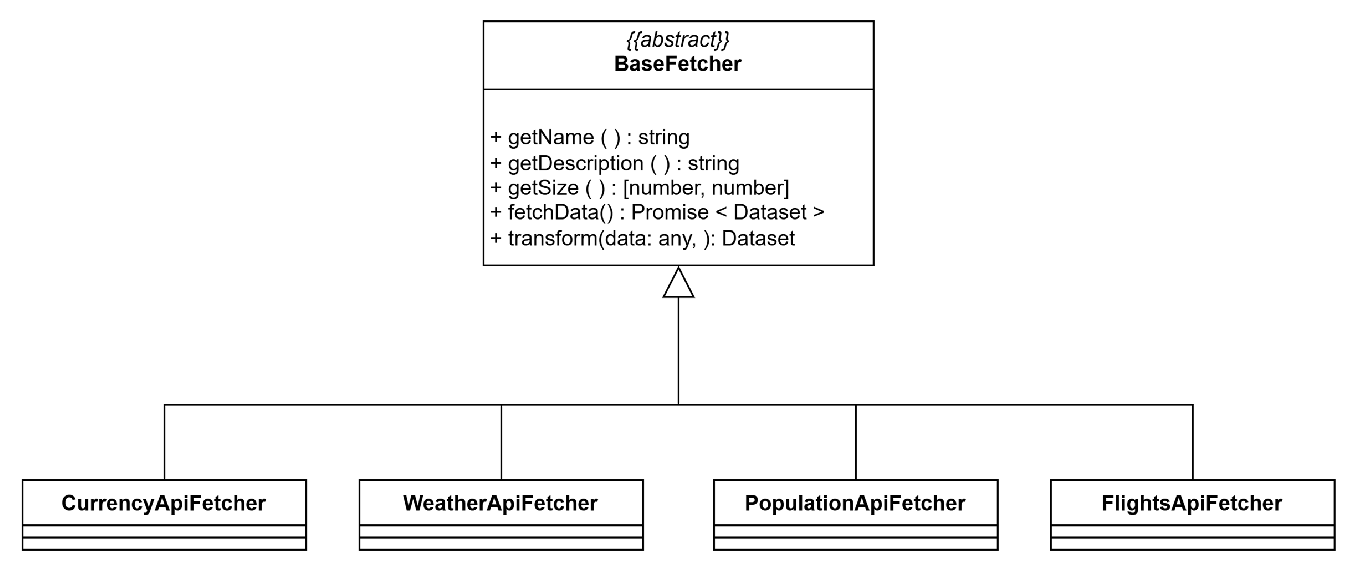
\includegraphics[scale = 0.55]{template/images/uml_back/Strategy.png}
    \caption{Pattern Strategy}
\end{figure}
Il \textbf{Design Pattern Strategy} è un pattern comportamentale che consente di definire una famiglia di algoritmi, incapsularli ciascuno in una propria classe e renderli intercambiabili all'interno di un contesto.
Questo approccio permette di variare dinamicamente l'algoritmo utilizzato da un oggetto, avendo diverse classi che differiscono solo per il comportamento, sono necessarie differenti varianti dello stesso algoritmo.
La classe \textit{BaseFetcher} definisce l'interfaccia per i fetcher dei dati, i suoi metodi vengono concretizzati poi nelle classi:
\begin{itemize}
    \item \textit{WeatherApiFetcher}
    \item \textit{FlightsApiFetcher}
    \item \textit{PopulationApiFetcher}
    \item \textit{CurrencyApiFetcher}
\end{itemize}
Nel nostro progetto abbiamo applicato il pattern Strategy per astrarre il comportamento di fetching dei dati da diverse sorgenti esterne.

